\documentclass{jsarticle}
\usepackage{color}
\usepackage{bm}
\usepackage[height=26cm,width=16cm]{geometry} 
\usepackage{amsmath}
\usepackage{cases}
\usepackage[dvipdfmx]{graphicx}
\title{確率論}
\graphicspath{{./image/}}

\begin{document}

\section{確率空間}
	\subsection{もっと数学的な定義}
		標本点:指向によって生じる個々の結果) \\
		根元事象:標本点1つの事象 \\
		標本空間:標本点の集合 集合 \\
		事象の集合F:標本空間Ωの部分集合族 $2^Ω$ \\
		部分集合族:部分集合の集合、べき集合 \\
		$F < 2^Ω$ である \\
		有限集合のときは$F = 2^Ω$\\
		事象:標本空間Ωの部分集合A、または、事象の集合Fの各要素 A ∈ F\\
		空事象:標本点を持たない事象\\
		確率測度:各事象に対して、0以上の数に対応させる実関数P\\
		確率空間:三つ組(Ω,F,P)を確率空間と呼ぶ ← 確率の世界的なもの\\
		\subsubsection{例}
			コイントスで、表をOとし、裏を1とする。 \\
			根元事象:「表が出る」→ {0} 「裏が出る」→ {1} \\
			標本空間:Ω={0,1}\\
			事象の集合:F=$2^Ω$=\{φ,\{0\},\{1\},\{1,0\}\} → できる集合全て、今回だと「何も取らない」「0または1だけ」「両方」\\
			確率測度:例えば、P(\{0\})=2/3 , P(\{1\})=1/3 , P(φ)=0 , P(\{1,0\})=1 → どっちかは必ず出る\\
		\subsubsection{同様に確からしい}
		n個の標本点からなる標本空間$Ω=\{ω_1,ω_2,....,ω_n\}$において、標本点$ω_i$のそれぞれが生起する確率が等しい時、すなわち \\
		$P(ω_1)=P(ω_2)= ... =P(ω_n)$\\
		が成り立つ時、「同様に確からしい」という。
		\subsubsection{例題2}
			コインを2枚投げた時、結果を(a,b)であらわす。\\
			根元事象:\{0,0\},\{(0,1)\},\{(1,0)\},\{(1,1)\}\\
			Ω=\{(0,0),(0,1),(1,0),(1,1)\}\\
			$F=2^Ω$個ある\\
			F=\{φ,\{(0,0)\},\{(1,0)\},\{(0,1)\},\{(1,1)\},\\
			\{(0,0),(0,1))\},\{(0,0),(1,0)\},\{(0,0),(1,1)\},\{(0,1),(1,0)\},\{(0,1),(1,1)\},\{(1,0),(1,1)\},\\
			\{(0,0),(0,1),(1,0)\},\{(0,0),(0,1),(1,1)\},\{(0,0),(1,0),(1,1)\},\{(0,1),(1,0),(1,1)\},\{(0,0),(0,1),(1,0),(1,1)\}\}\\
	\subsection{確率の公理的定義}
		コルモゴロフの定義 \\
		公理1:全ての要素Eiに対して 0≦P(Ei) である\\
		公理2:P(Ω)=1 \\
		公理3:お互いに排反な事象Eiにたいして、$P(\bigcup^∞ _{i=1} Ei) = \sum_{i=1}^∞ P(E_i)\\$
		※「互いに排反な事象$E_i$とは\\
		すべてのn≠mに対して\\
			$E_n ∩E_m = φ$ \\
		が成り立つこと\\
		\\
		公理1~3を満たさなければ、確率とは言えない。\\
		公理から次が導き出される\\
		1. P(φ)=0\\
		2 . 単調性:A ⊆ Bならば、P(A) ≦ P(B)\\
		3 . 上界:$0 ≦ P(A_i) ≦ 1$ \\
		4 . 加法定理 P(A ∪ B) = P(A) + P(B) - P(A ∩ B)\\
		5 . 余事象の法則 $P(A^c) = 1-P(A)$
		
		******宿題 公理1~3のみを用いて、1〜5の関係が成り立つことを示せ。A/Bはつかう??
\section{確率変数と確率分布}
	離散変数の場合を考える
	\subsection{確率変数}
	定義 ( いくつかある)\\
	1 . 確率変数とは、試行する実験結果として取り得る値を表す変数  サイコロ 1〜6 \\
	2 . 事象Xが確率を伴った出現する時、Xを確率変数と呼ぶ \\
	3 . 標本空間Ωの各要素に対して、実数の集合Rの1つの値を割り当てる関数として、確率変数Xを定義する \\
	X:Ω → R \\
	y=f(x) x,yは変数 f:R→R \\
	※「事象を数値で表したもの」を確率変数とする \\
	確率変数は大文字のXで表し、その実現値は小文字で表す \\
	サイコロ\\
	   確率変数をXとする。 \\
	   P(X=1),P(X=2), .... ,(P(X=6)) \\
	   P(X)=x \\

\section{10/19 : }
	前回.三つ組(Ω,F,P)ですべての確率を表すことができる\\
	\subsection{離散確率分布}
		{\bf{確率分布とは}} ・・・ \\
		各事象Jに対して、それが起こる確率を割り当てたもの。つまり、確率測度を定義したものである。\\
		確率分布表やグラフ、数式で与えることができる。\\
	\subsection{例題}
		{\bf{コイントス}}
		\begin{center}
			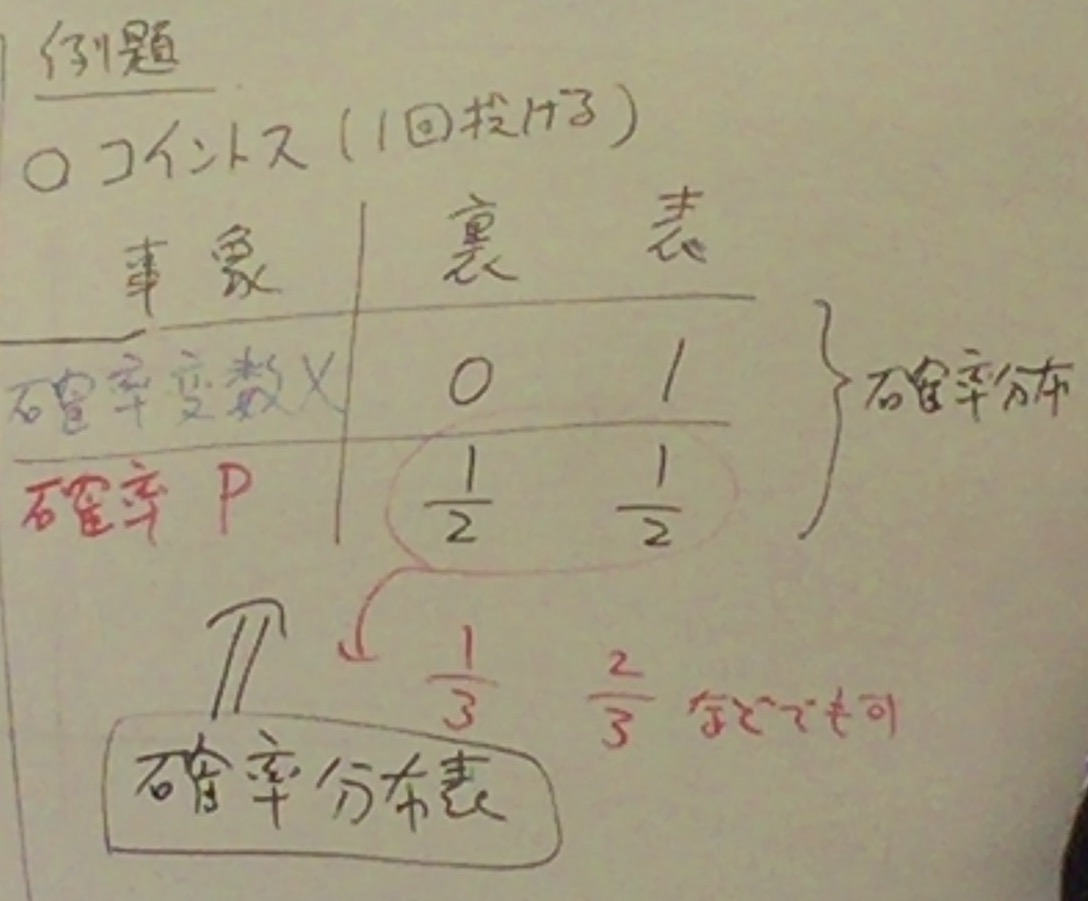
\includegraphics[width=5cm]{10_19_1.JPG}
		\end{center}
		
		{\bf{2つのサイコロ}}\\
		2つのサイコロを投げた時、出た目の数をXとYで表す\\
		※XとYはそれぞれ確率変数\\
		「出た目の和」を考えたい\\
		和X+Yも確率変数である\\
		\begin{center}
			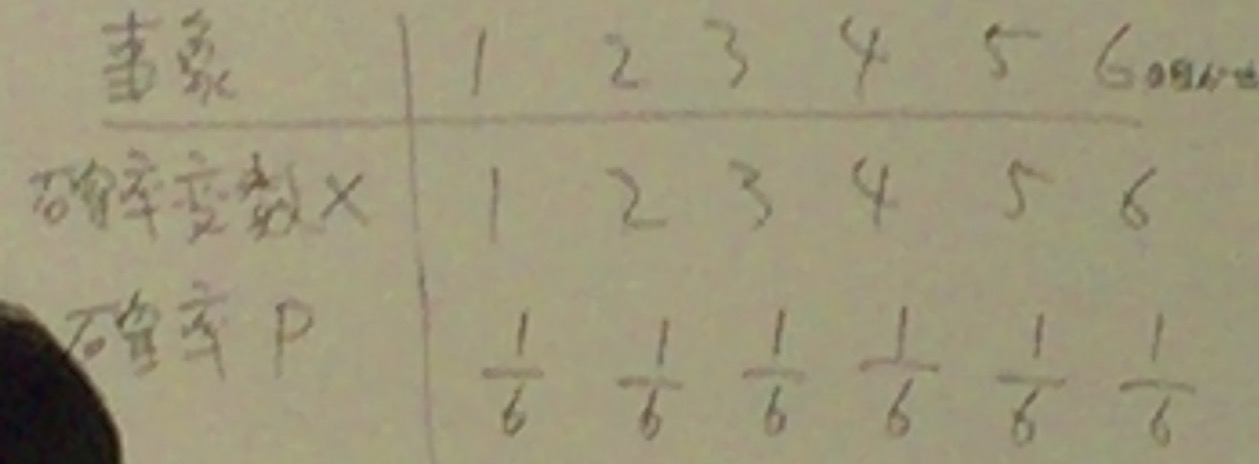
\includegraphics[width=5cm]{10_19_2.JPG}
		\end{center}
		
		和X+Yの確率分布
			
		\begin{center}
			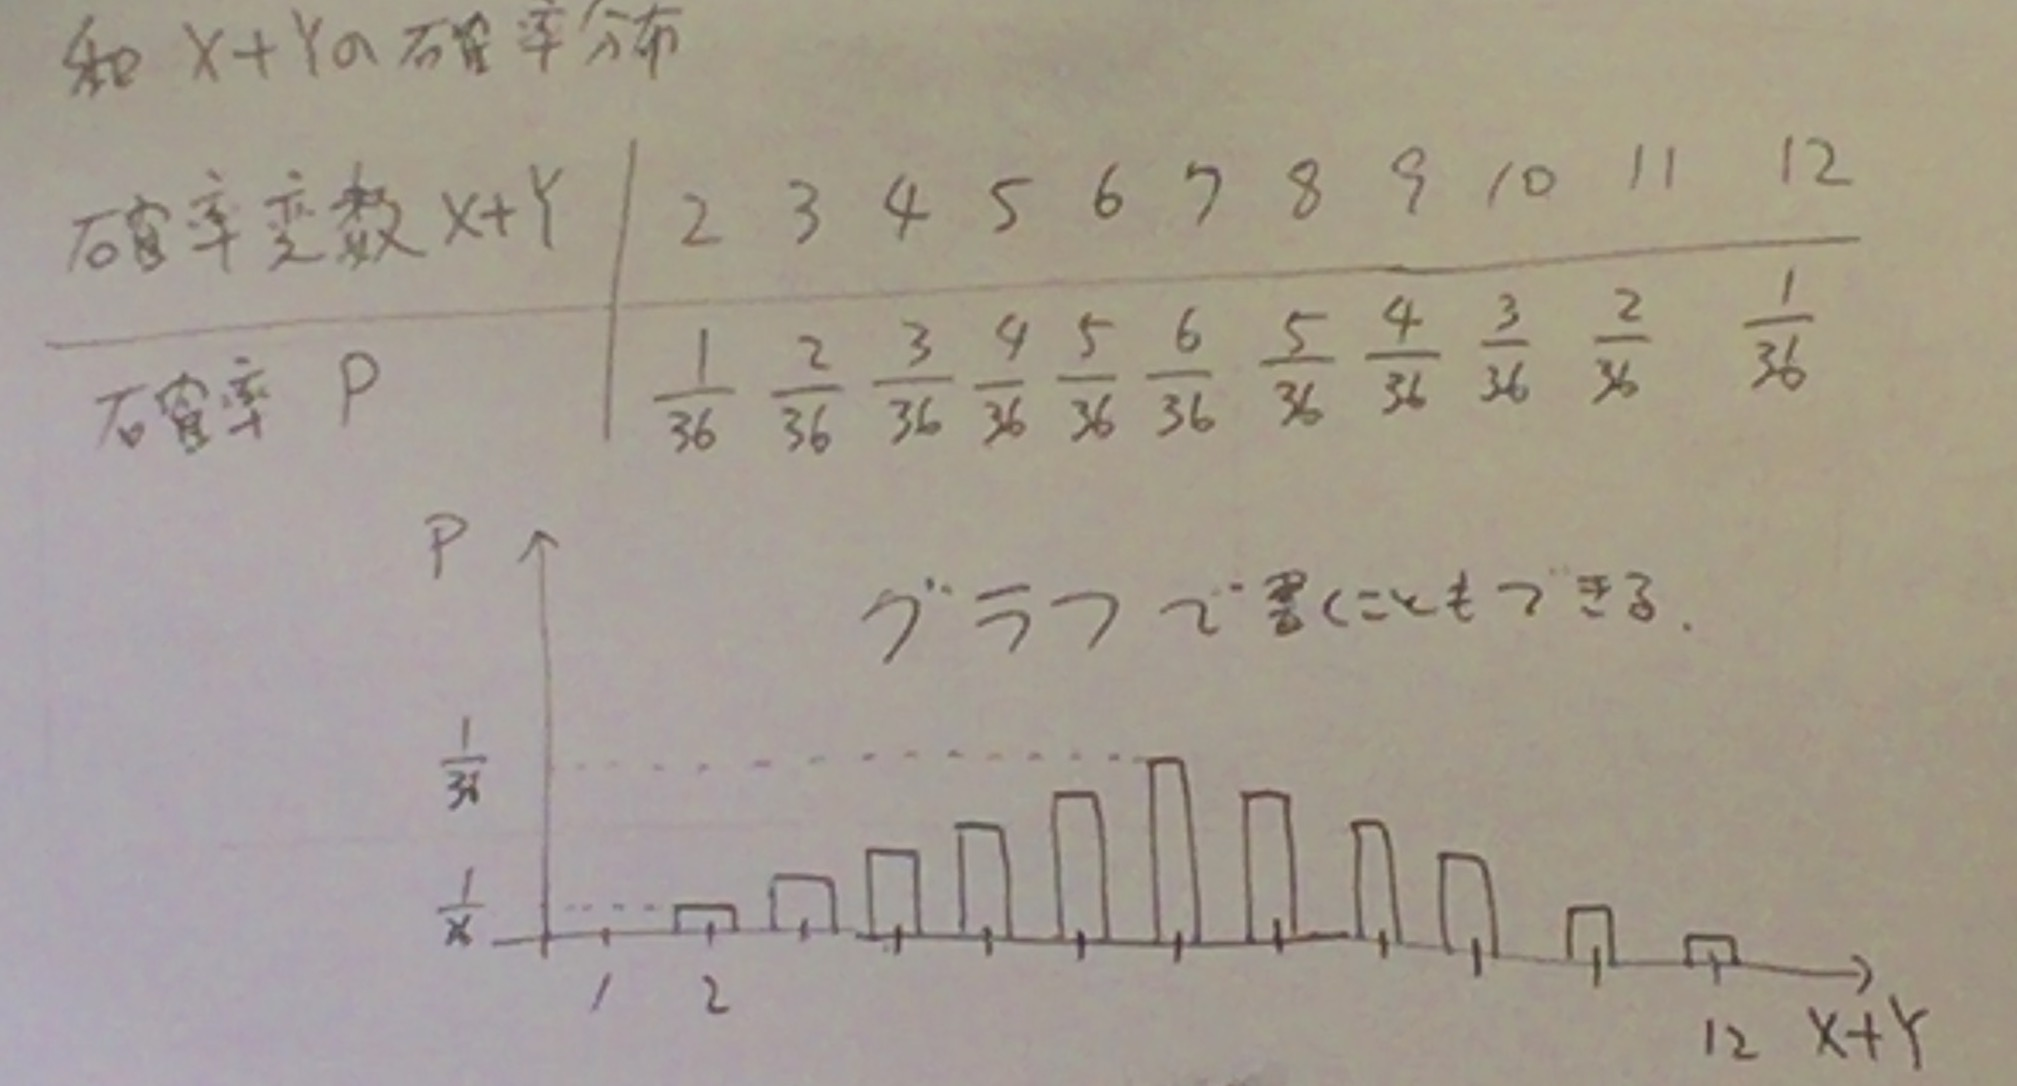
\includegraphics[width=10cm]{10_19_3.JPG}
		\end{center}
		確率分布が数式で表せる場合\\
		{\bf{離散一様分布}}\\
		n個の事象が等しく起こる確率分布\\
		$P(X=r)=\frac{1}{n} ,\ \  r=1,2,3,....,n$\\
		$P(X=r)はP(r),P_x(r)$と書くこともある\\
		↑「確率変数Xがrとなる確率」\\
		\subsubsection{例:サイコロ}
			サイコロの目がrとなる確率\\
			$P(X=r)=\frac{1}{6}$ \\
			
	\subsection{二項分布}
		確率pで起こる事象が、n回の試行中 r回起こる確率分布\\
		$P(X=r)=P_x(r)={}_n C _r P^r(1-P)^{n-r} $\\
		
		\subsubsection{例:n回のコイントス}
			コインを10回投げた時表が3回出る
			$P(X=3)={}_{10}C_3 (\frac{1}{2})^3(1-(\frac{1}{2})^{10-3})$
			
	\subsection{ポアソン分布}
		単位時間中に平均でλ回起こる事象がk回起こる確率分布 \\
		$P(X=r)=\frac{λ^k}{k!} e^{-λ}$
		
	\subsection{連続確率分布}
	確率変数が連続値(実数)をとる場合
	\begin{center}
			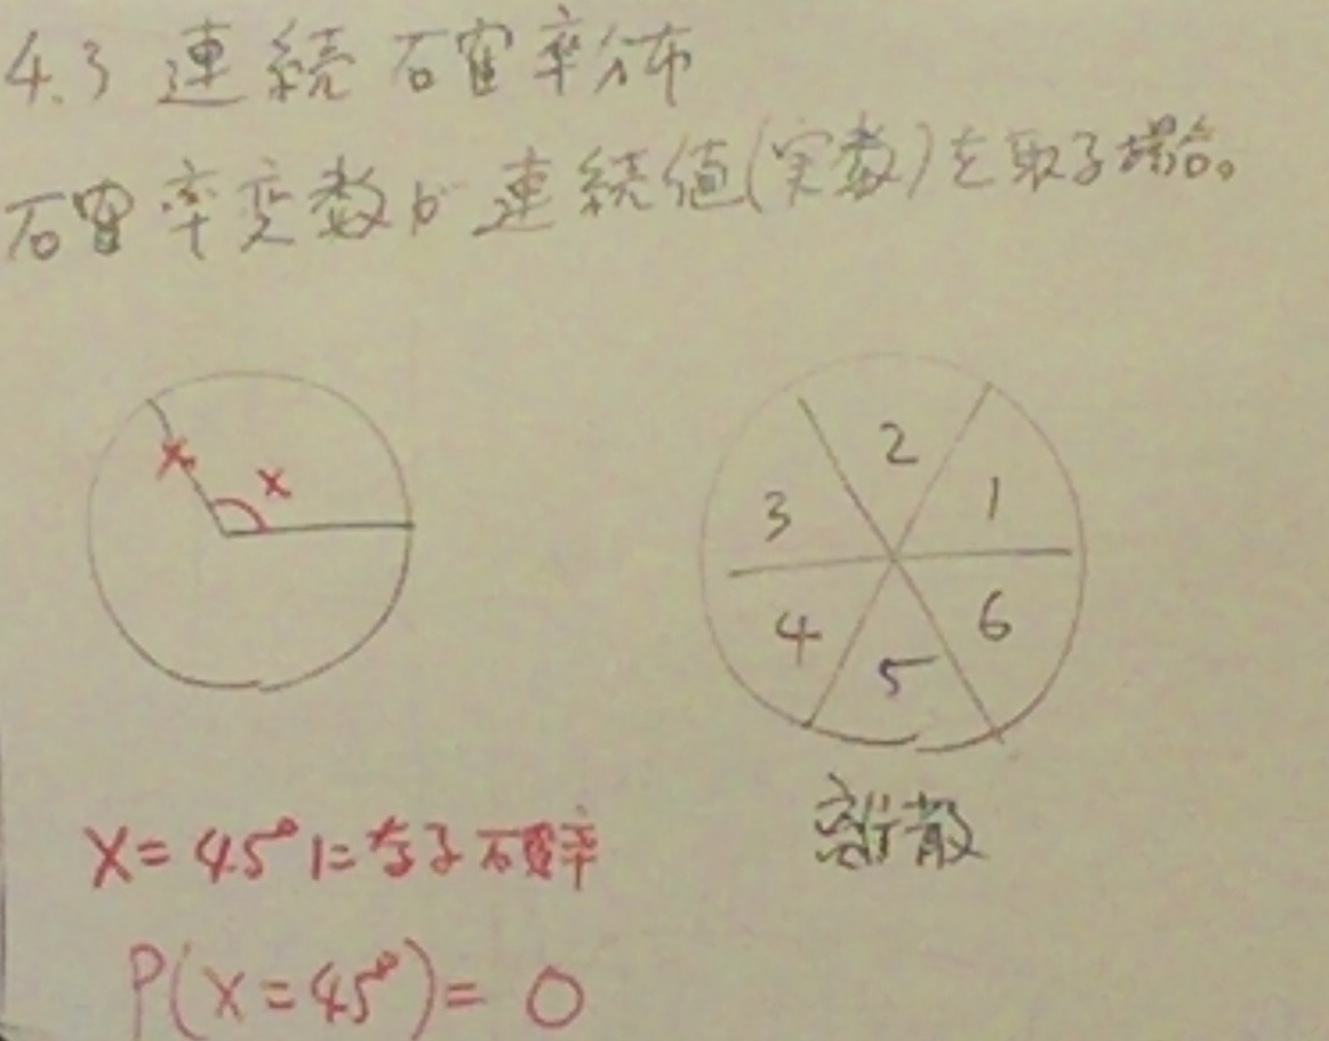
\includegraphics[width=10cm]{10_19_4.JPG}
	\end{center}
	
	連続確率分布のときは、ある値rを取り確率は0であることが多い。\\
	↓\\
	{\bf{「X=rとなる確率」}}には意味はない\\
	$「a≦x≦bとなる確率」$を考えることができる\\
	
	\subsubsection{定義}
		確率変数Xに対して、$a≦x≦b$となる確率が\\
		\[
 			P(a≦x≦b)= \int_a^b f(x) dx
		\]
		で与えられる時、$f(x)$を\\
		{\Large{\bf{確率密度関数}}}\\
		と定義する。\\
		ただし、$f(x)≧0$とする\\
		
		全区間で積分すると\\
		\[
			\int_a^b f(x) dx =1
		\]
		である\\
		※$f(x)$の値は1を超えることもある\\
		
		連続系の場合は、{\bf{確率密度関数}}を考える\\
		※確率密度関数であることの必須条件\\
		\begin{enumerate}
			\item $f(x) ≧ 0$
			\item $\int^∞_{-∞}f(x) dx =1$
		\end{enumerate}
		$f(x)$が確率密度関数ならば、1と2を満たす\\
		
	\subsubsection{例題}
		区間[0:1]において、$f(x)=x$は確率密度関数の必要条件を満たすか?\\
		
		\begin{enumerate}
			\item $f(x) ≧ 0$は満たす($0≦x≦1)$ 
			\item $\int^∞_{-∞} f(x) dx = \int^1_0 x dx = 1/2 ≠ 1$
		\end{enumerate}
		
		これより、$f(x)=x$は必要条件を満たしていない
	
	\subsubsection{連続確率分布}
		 連続一様分布 \\
		 区間[a:b] で一様である時
		 \[
		 	f(x) = 
		 	\begin{cases}
			 	{}
			 	\frac{1}{b-a} & a≦x≦b\\
			 	0  & その他
			\end{cases}
		\]
	\subsubsection{正規分布(ガウス分布)}
		平均μ,分散$σ^2$ の正規分布
		\[
			f(x)=\frac{1}{\sqrt{2π}r}e^{-\frac{(x-μ)^2}{2σ^2} }\\
		\]
	
	\subsubsection{指数分布}
		単位時間当たりにλ回起こる事象が怒った後つぎに発生するまでの生起間隔がx単位時間である確率
		\[
			f(x) = 
			\begin{cases}
  				λe^{-λx} & x≧0 \\
				0
			\end{cases}
		\]
		
	\subsubsection{ガンマ分布}
	\[
		f(x)=x^{k-1}\frac{e^{-\frac{x}{θ}}}{Γ(k)θ^k} \ (x≧0)
	\]
	$Γ(k)$はガンマ関数
	\[
		Γ(k)=(k-1)!
	\]
		\begin{center}
			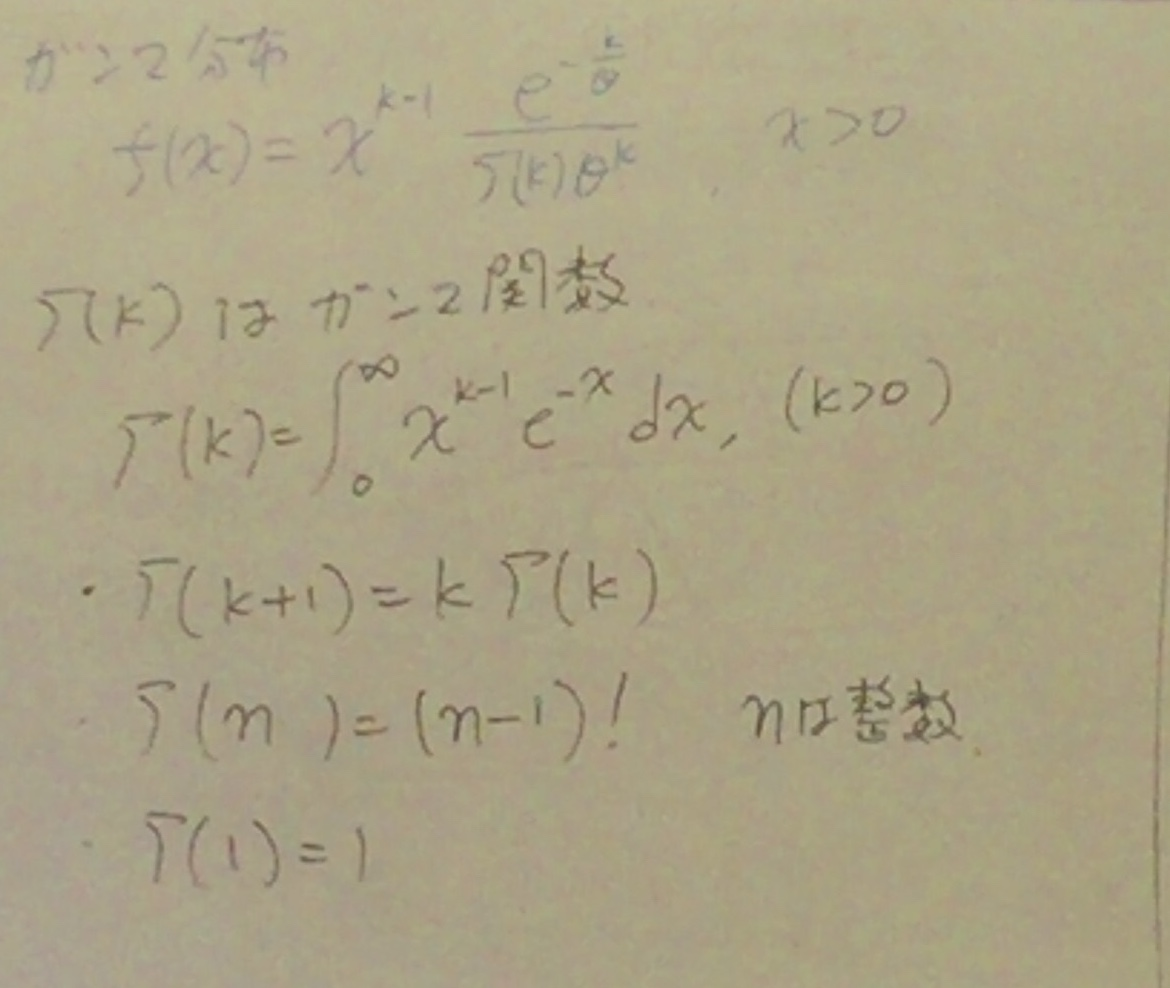
\includegraphics[width=10cm]{10_19_5.JPG}
		\end{center}
		********宿題。。。画像
\section{10/26}

	\subsection{累積分布関数}
	\bf{累積分布関数F(x)} ・・・ ある値がx以下である確率$P(X ≦ x)$
	\[
		F(x)=P(X ≦ x)
	\]
	と定義する \\
	連続型確率変数の場合 \\
	\[
		F(x)=\int^x_{-∞} f(u) du
	\]
	\begin{center}
		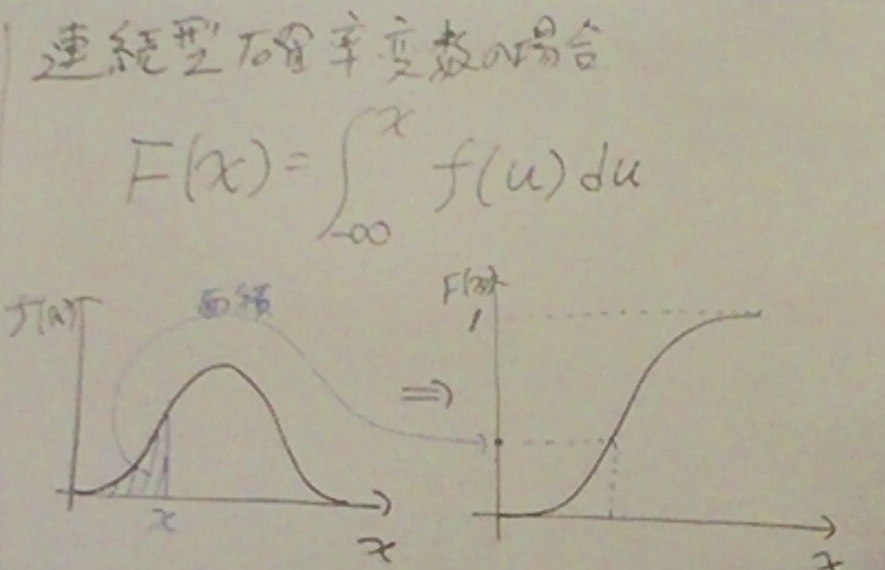
\includegraphics[width=10cm]{10_26_1.JPG}
	\end{center}
		
	\subsection{期待値と分散}
	確率分布の特徴を考えてみる\\
	\bf{代表値} \\
	・平均値(average) : 標本平均。全てのデータの総和をデータ数で割ったもの \\	
	・中央値(median) : データを大きさ順に並べた時、真ん中に来る値のこと \\
	・最頻値(mode) : 最もデータ数が多い値のこと\\
		\subsubsection{例 }
			データ(1,1,2,4,5,8,9,10,11)
			平均値=5.66\\
			中央値=5番目が真ん中=5\\
			最頻値=1\\
			
	\subsection{期待値}
		期待値は、ある確率分布の平均的な値を知る尺度である\\
		
		\subsubsection{理論的期待値}
			離散確率空間$(Ω , F , P)$において、標本空間Ωが
			\[
				\Omega=\{x_1,x_2, ... ,x_n\}
			\]
			であり、この確率空間上の確率変数を$X$とする\\
			このとき、確率変数$X$の期待値$E$(エクスペクテーション)は
			\[
				E[x]=\sum^n_{i=1}x_iP(X=x_i)
			\]
			で定義する\\
			定義だから覚える\\
			※$P(X=x_1)$を$P_i$と略すことがある	\\
			連続確率空間に対しては、確率変数Xの期待値は、確率密度関数$f(x)$を用いて
			\[
				E[x]=\int^∞_{-∞} xf(x)dx
			\]
			で定義する
			
		\subsubsection{例題}
			10本のくじがある。A賞が当たると1000円、B賞は500円、C賞は100円もらえるとする。\\
			ただし、各賞はA賞2本、B賞は3本、C賞は5本入っている。\\
			くじを1回引いた時、いくら貰えると期待できるか。\\
			とりあえず確率分布表を書こう\\
			
			\begin{center}
				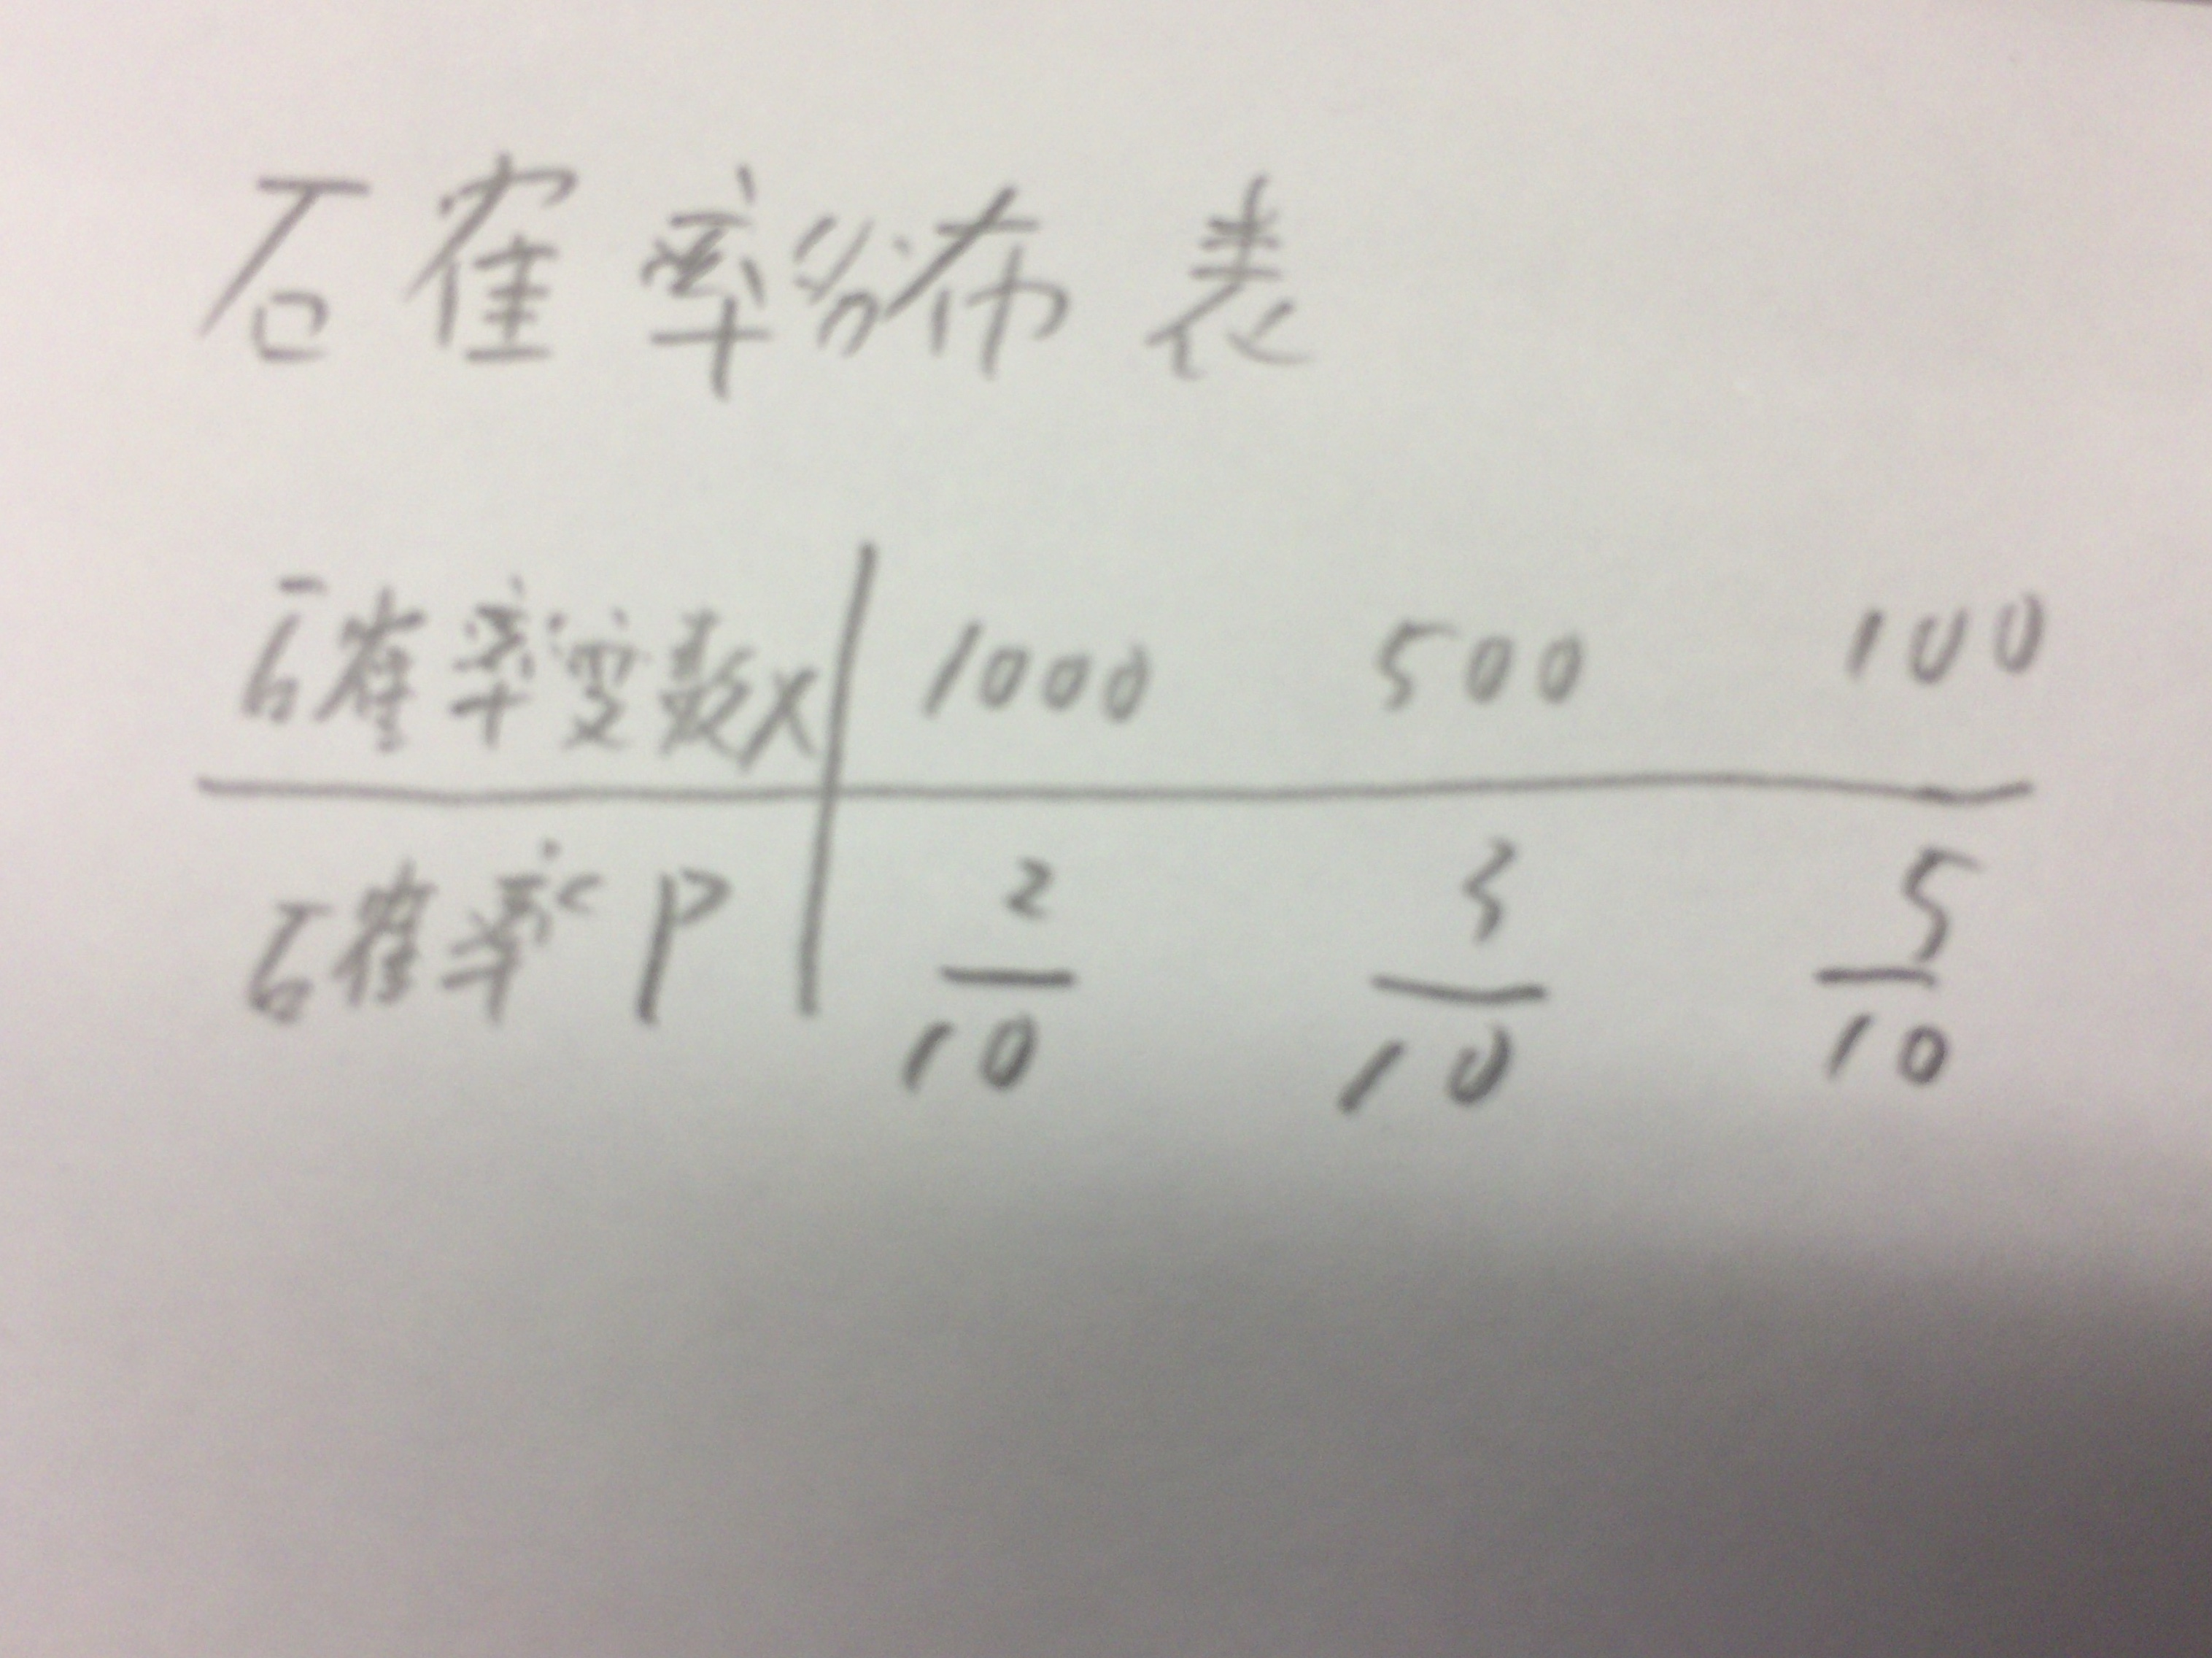
\includegraphics[width=5cm]{10_26_2.JPG}
			\end{center}
			
			標本空間$\Omega$
			\[
				\Omega=\{x_1=1000 , x_2 = 500 , x_3=100\}
			\]
			確率測度P
			\[
				P_1=P(X=x_1)=\frac{2}{10}, P_2=P(X=x_2)=\frac{3}{10} , P_3=P(X=x_3)=\frac{5}{10}
			\]
			期待値
			\[
				E[x]=\sum^3_{i=1}x_iP(X=x_3)
					=1000×2/10+500*3/10+100*5/10
					=400
			\]
			1回当たり400円貰えると期待できる
	\subsection{分散}
		
		******もしかしたらxとXがごちゃごちゃになってる??\\
		ある確率分布の値のばらつきは分散または標準偏差で測ることができる。\\
		分散と標準偏差\\
		確率変数Xの期待値を$μ=E[x]$とするこXの分散$σ^2$は
		\[
			σ^2=V[X]=E[(x-μ)^2]
		\]
		で定義される
		また、σを標準偏差と呼ぶ
		\[
			σ=\sqrt{V[X]}
		\]
		\begin{center}
			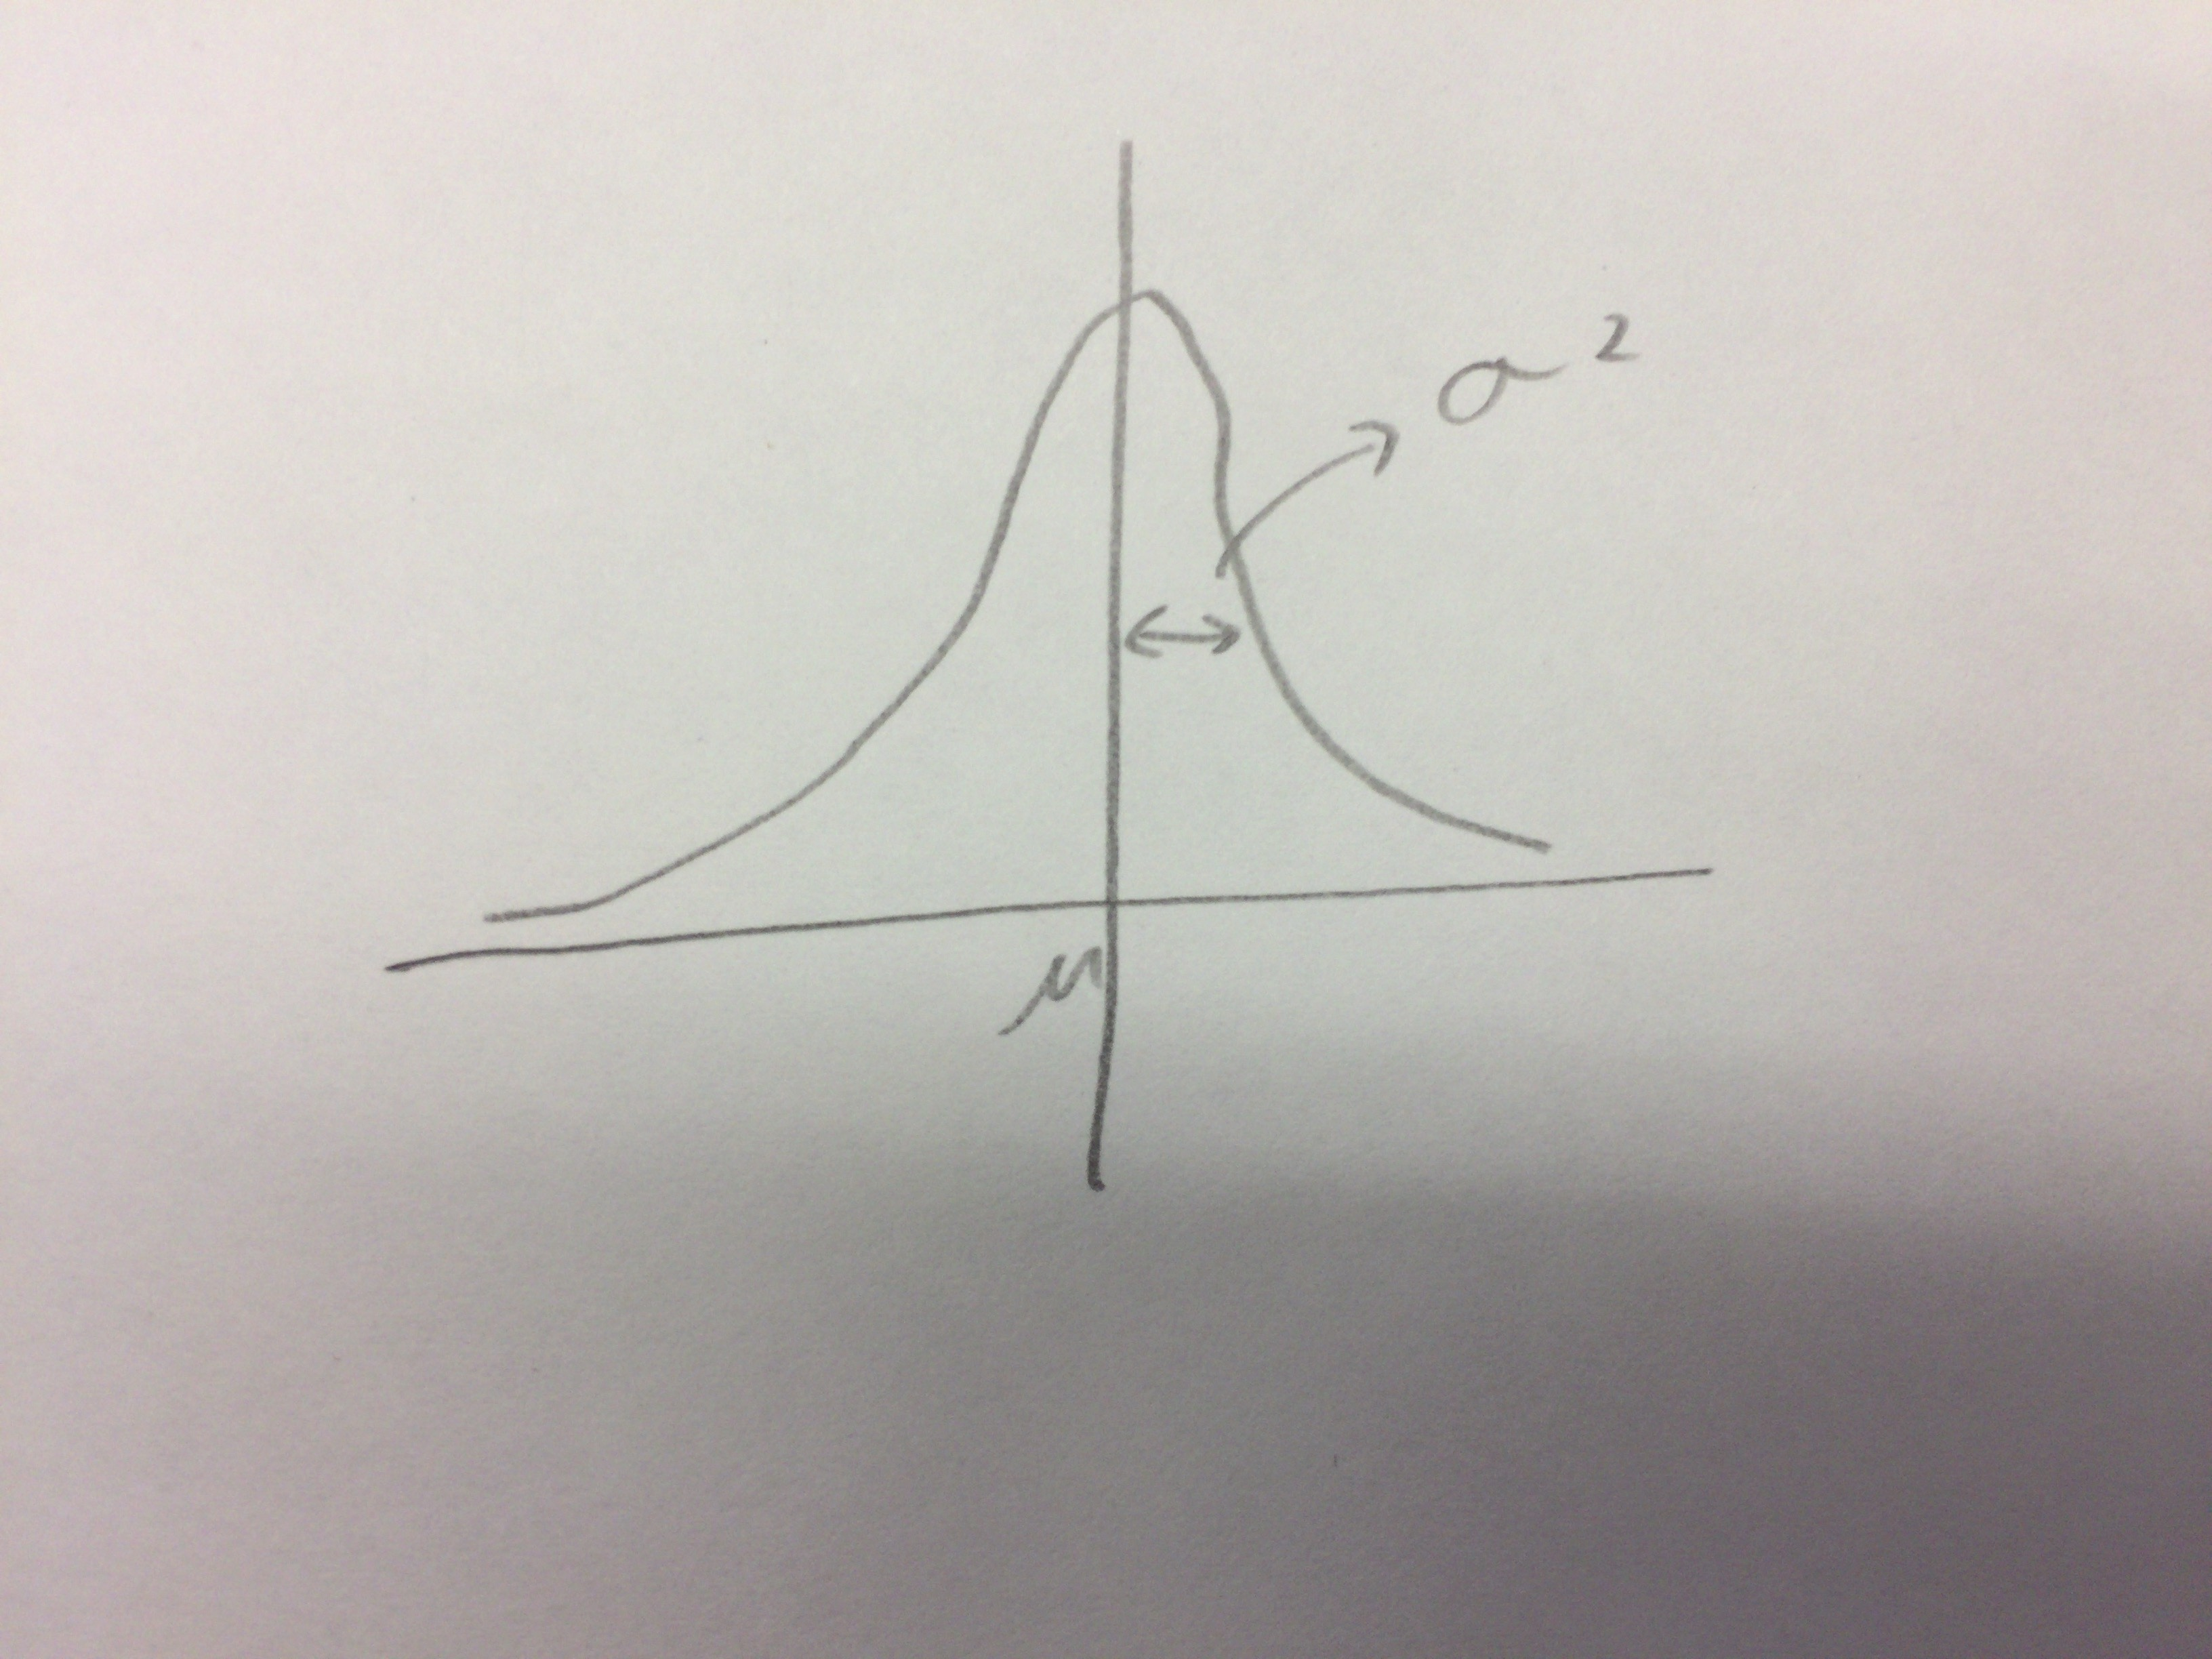
\includegraphics[width=5cm]{10_26_3.JPG}
		\end{center}
		
		離散確率空間(Ω , F , P)において
		\[
			\Omega={x_1,x_2,....,x_n}
		\]
		であり、この確率空間上の確率変数をXとする\\
		このとき、確率変数Xの分散は
		\[
			V[X]=\sum^n_{i=1}(x_i-μ)^2P(X=x_i)
		\]
		
		同様に連続確率空間では
		\[
			V[X]=\int^∞_{-∞} (x-μ)^2f(x)dx
		\]
		で定義する\\
		{\Large{分散の公式}}
		\[
			V[X]=E[X^2]-(E[X])^2
		\]
		*******宿題この式を示せ
	\subsection{計算公式}
		確率変数X、Yと、定数a,b,c において\\
		E1 : $E[c]=c$\\
		E2 : $E[aX+b]=aE[X]+b $\\
		E3 : $E[X+Y]=E[X]+E[Y]$\\
		V1 : $V[c]=0$\\
		V2 : $V[X+c]=V[X]$\\
		V3 : $V[cX]=c^2V[X]$\\
		V4 : $V[X±Y]=V[X]+V[Y]$→ただし、XとYは互いに独立であるとする\\
		分散にマイナスはない\\
		{\Large{独立・・・}}\\
		お互いの結果が、影響し合わないこと
		\[
			P(X\cap Y)=P(X)P(Y)
		\]
		\subsubsection{練習問題}
			1.サイコロを1回降った時、出る目の期待値μと分散$σ^2$を求めなさい\\
			標本空間Ω\\
			$Ω=\{x_1=1,x_2=2 ,... ,x_6=6\}$\\
			確率測度\\
			$P_1=P_2=...=P_6=1/6$\\
			出る目の値を確率変数Xとおく\\
			\[
				μ=E[X]=\sum^6_{i=1}x_iP_i
				=1*1/6+2*1/6+....+6*1/6
				=3.5=7/5
			\]
			分散$σ^2$
			\[
				σ^2=V[X]=\sum^6_{i=1}(x_i-μ)^2P_i
			\]
			もしくは
			\[
				E[X^2]=\sum^6_{i=1}x^2P_i
				=91/6
			\]
			これより
			\[
				V[X]=E[X^2]-(E[X])^2=91/6-(7/2)^2=35/12
			\]
			
\section{11/21}
\subsection{高次の統計量}
	\subsubsection{m次モーメント}
		期待値$μ=E[X]$のまわりのm次モーメント\\
		$μ_m , m=1,2,3,...$を
		\[
			μ_m=E[(X-μ)^m]=\sum^m_{i=1}(x_i-μ)^mP(X=x_i)
		\]
		と定義する\\
		分散$σ^2$は2次モーメントに等しい\\
		\[
			σ^2=μ_2
		\]
		
	\subsubsection{歪度}
		分布の歪み度をあらわす尺度
		\[
			β_1=\frac{μ_3}{σ^3}=\frac{E[(X-μ)^3]}{σ^3}
		\]
		σ:標準偏差\\
		・$β_1=0$のとき、期待値μを中心に左右対称になる\\
		・$β_1>0$のとき、中心よりも左に歪んだ分布になる\\
		・$β_1<0$のとき、中心よりも右に歪んだ分布になる\\
		
		\begin{center}
			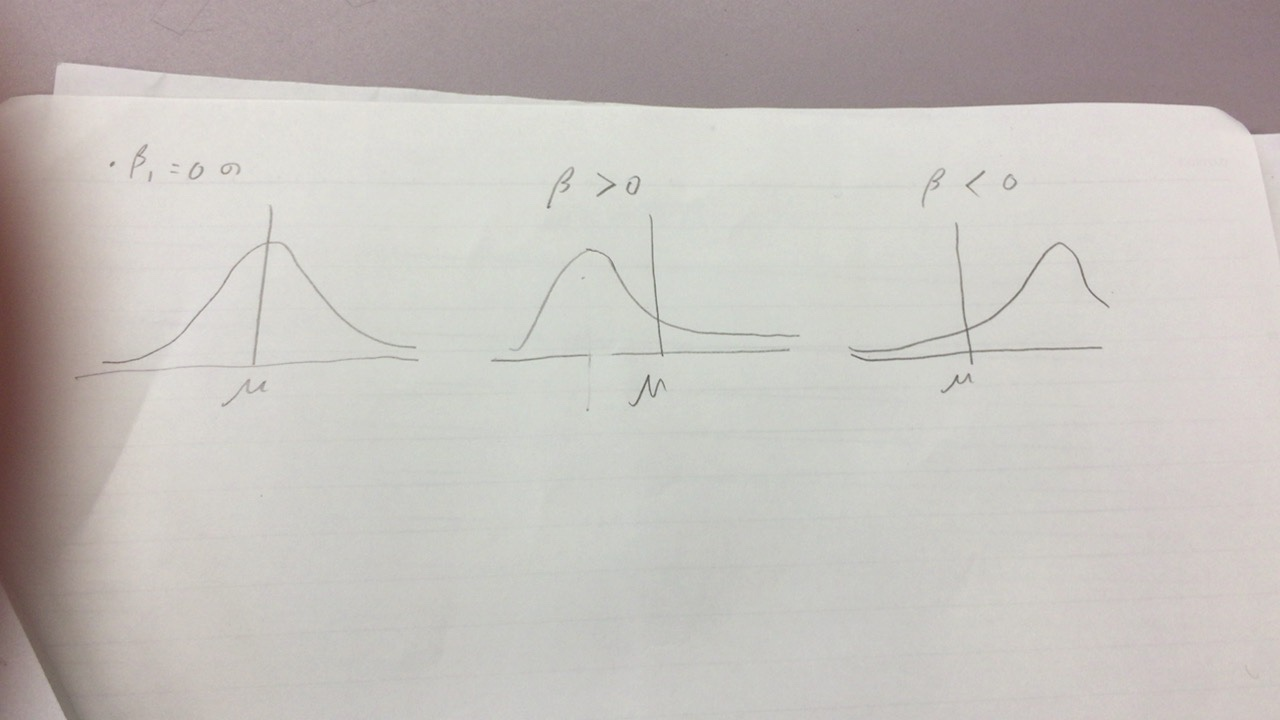
\includegraphics[width=10cm]{11_2_1.JPG}
		\end{center}
	\subsubsection{尖度}
		分布の尖り度を表す尺度である
		\[
			β_2=\frac{μ_4}{σ^4}-3=\frac{E[(X-μ)^4}{σ^4}-3
		\]
		・$β_2$が大きい時\\
		鋭いピークと太く長い裾を持つ
		・$β_2$がちいさいとき\\
		丸みがかかったピークで、短く細い裾を持つ
\subsection{様々な確率分布}
	\subsubsection{ベルヌーイ分布}
		・ベルヌーイ試行・・・・\\
		1回の試行で、2つの結果AまたはBが起こる実験をベルヌーイ試行と呼ぶ\\
		例\\
			・コインを1枚1回投げる試行\\
			・ある病気である、または、ある病気でない\\
		事象AとBに対して、確率変数Xを用いてそれぞれ1,0で表す\\
		1が出る確率を$p$で表す\\
		ベルヌーイ分布
			\begin{numcases}
			{}
				P(X=1)=p\\
				P(X=0)=1-p
			\end{numcases}
		確率変数Xはパラメータ$p$のベルヌーイ分布$Be(p)$に従うという\\
		\[
			X〜Be(p)
		\]
		期待値:$E[X]=p$
		分散:$V[X]=p(1-p)$
		
	\subsubsection{二項分布}
		ベルヌーイ試行をn回行った時、結果Aが怒る回数Xは確率変数となる\\
		二項分布B(n,p):離散分布\\
		確率pで結果Aが怒る試行において、n回行った時、ちょうどk回怒る確率は\\
		\[
			P(X=k)={}_nC_k p^k(1-p)^{n-k}
		\]
		\[k=0,1,2,3..\]
		で与えられる\\
		確率変数Xはパラメータ$n,p$の二項分布$B(n,p)$に従うという\\
		\[
			X〜B(n,p)
		\]
		\subsubsection{例題}
			表が出る確率が$p=\frac{3}{5}$である曲がったコインを5回投げた時、表が3回出る確率はいくらか\\
			\[
				P(X=3)={}_5C_3p^3(1-p)~{5-3}=10*(3/5)^3*(2/5)^2=\frac{216}{625}
			\]
			k=0,1,2,3,4,5の場合について計算すると、確率分布表がかける
			\begin{center}
				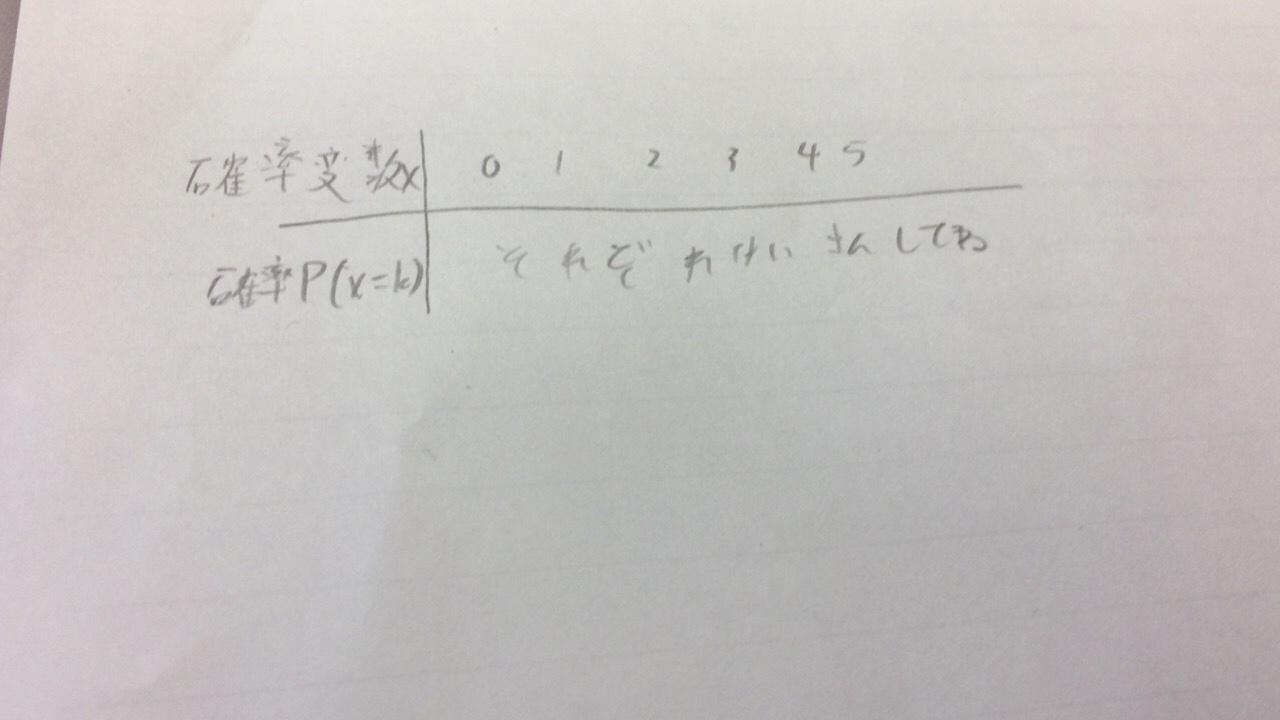
\includegraphics[width=10cm]{11_2_2.JPG}
			\end{center}
		
		B(n,p)の特徴\\
		期待値E[X]=np\\
		分散V[X]=np(1-p)\\
		※二項定理
			
		\subsubsection{ポアソン分布$P_o(λ)$:離散分布}
			単位時間あたりにλ会起こる事象がk回起こる確率は
			\[
				P(X=k)=\frac{λ^k}{k!}e^{-λ}
			\]
			で与えられる。$λ>0$とする\\
			確率変数Xはパラメータλのポアソン分布$P_o(λ)$に従うという
			\[
				X〜P_o(λ)
			\]
			\subsubsection{例題}
				1時間あたりにλ=3回メールが届く人がいる。→単位時間あたりだからポアソン\\
				この人がk=5回メールを受信する確率はいくらか
				\[
					P(X=5)=\frac{3^5}{5!}e^{-3}=0.1008
				\]
				
				
				ポアソン分布の特徴\\
				期待値$E[X]=λ$\\
				分散 $V[X]=λ$
		\subsubsection{指数分布:連続分布}
			パラメータ$λ>0$を持つ確率密度関数
			\begin{numcases}
				f(x)={}
					λe^{-λx} ,& $x≧0$\\
					0             ,& $x < 0$
			\end{numcases}
			で与えられる確率分布を、指数分布という\\
			
				
			確率変数Xはパラメータλの指数分布に従うという
			\[
				X〜E_xp(λ)
			\]
			\subsubsection{例題}
			・地震が起こる間隔\\
			地震が起きてから次に起こるまでの時間\\
			・メールを受信する間隔\\
			※ポアソン分布との違い
			
			単位時間あたり平均λ回起こる現象に対して\\
			・単位時間に事象が起こる回数$〜P_o(λ)$\\
			・事象の発生間隔は平均$\frac{1}{λ}$の指数分布に従う\\
		
			指数分布の特徴\\
			期待値$E[X]=\frac{1}{λ}$ ← 部分積分 \\
			分散$V[X]=\frac{1}{λ^2}$\\
			
			*************宿題\\
			二項分布、ポアソン分布、指数分布の期待値と分散を導出しなさい\\

\section{11/9}
\subsection{正規分布(連続分布)}
	平均μ,分散$σ^2$をもつ確率密度関数
	\[
		f(x)=\frac{1}{\sqrt{2πσ^2}}e^{-\frac{(x-μ)^2}{2σ^2}}
	\]
	で定められる確率分布を正規分布という
	\[
		=\frac{1}{\sqrt{2πσ^2}exp[-\frac{(x-μ)^2}{2σ^2}}]
	\]
	確率変数Xは、平均μ、分散$σ^2$の正規分布に従うという
	\[
		X〜Ν(μ,σ^2)
	\]
	※ガウス分布ということもある\\
	
	正規分布の特徴 \\
	期待値 
		\[
			E[X]=μ
		\]
	分散
		\[
			V[X]=σ^2
		\]
	{\large{標準正規分布N(0,1)}}\\
	平均μ=0,分散$σ^2=1$であるとき恭順正規分布という\\
	$Ν(μ,σ^2)$に対して、\\
	\textcolor{blue}{標準化変数
	\[
		z=\frac{x-μ}{σ}
	\]
	}
	を導入する\\
	zは標準正規分布N(0,1)に従う\\
	\[
		Z〜N(0,1)
	\]
	\begin{center}
		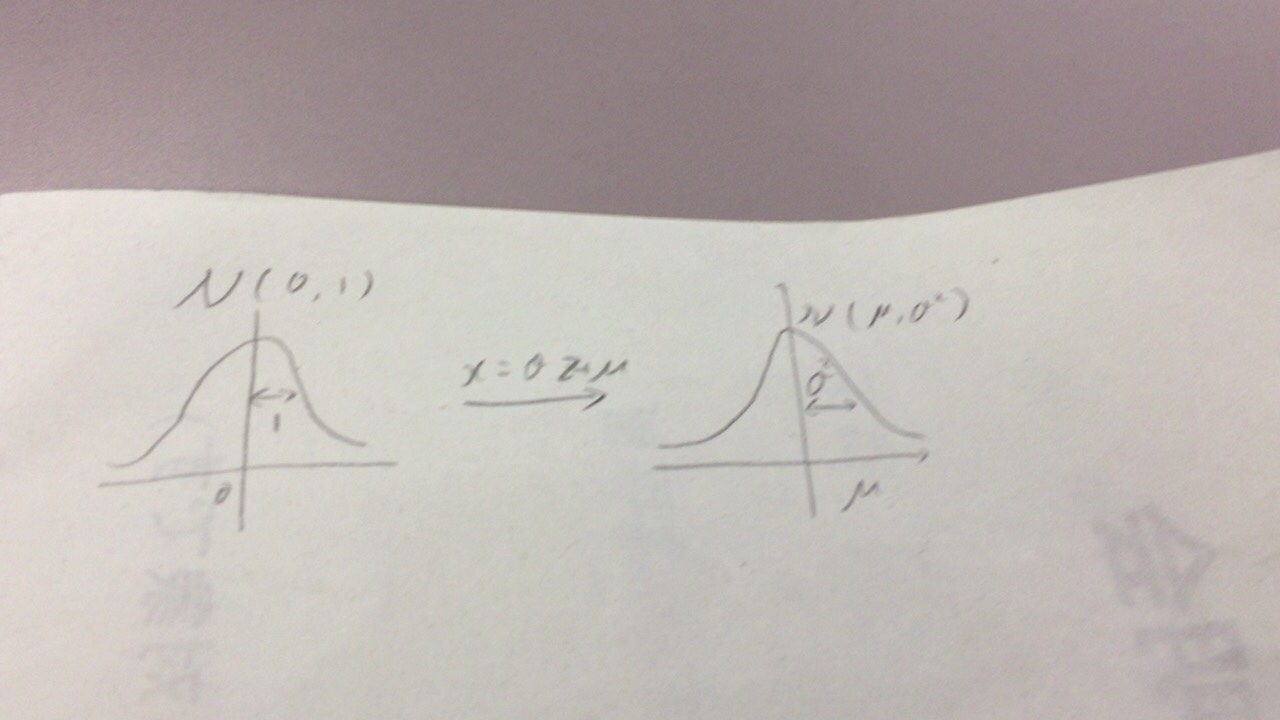
\includegraphics[width=5cm]{11_9_1.JPG}
	\end{center}
	\subsubsection{累積分布関数}
		\[	
			F(x)=P(X≦x)=\int^x_{-∞}f(u) du
		\]
		標準正規分布の場合
		\[
			Φ(x)=\frac{1}{\sqrt{2π}}\int^x_{-∞}e^{-\frac{u^2}{2}}du
		\]
	\subsubsection{チェビシェフの不等式}
		期待値μからの標準偏差σの単位で、k倍以内になる確率は
		\[
			P(|X-μ|≦kσ|)>1-\frac{1}{k^2} 
		\]
		である\\
		ある確率分布\\
		2σ以内$1-\frac{1}{2^2}=75\%$以内\\
		3σ以内$88\%$以内\\
		より大きい\\
		正規分布の場合\\
		2σ以内$95\%$以内\\
		3σ以内$99.7\%$以内\\
		より大きい(正規分布のは覚えといたほうがいい??)\\
	\subsubsection{誤差関数とQ関数}
		誤差関数$erf(x)$\\
		\[
			erf(x)=\frac{2}{\sqrt{x}}\int^x_0e^{-t^2}dt
		\]
		相補誤差関数$erfc(x)$\\
		\[
			erfc(x)=1-erf(x)=\frac{2}{\sqrt{π}}\int^∞_xe^{-t^2}dt
		\]
		{\large{Q関数}}
		\[
			Q(x)=\frac{1}{2}[1-erf(\frac{2}{\sqrt{2}})
		\]
		\begin{center}
			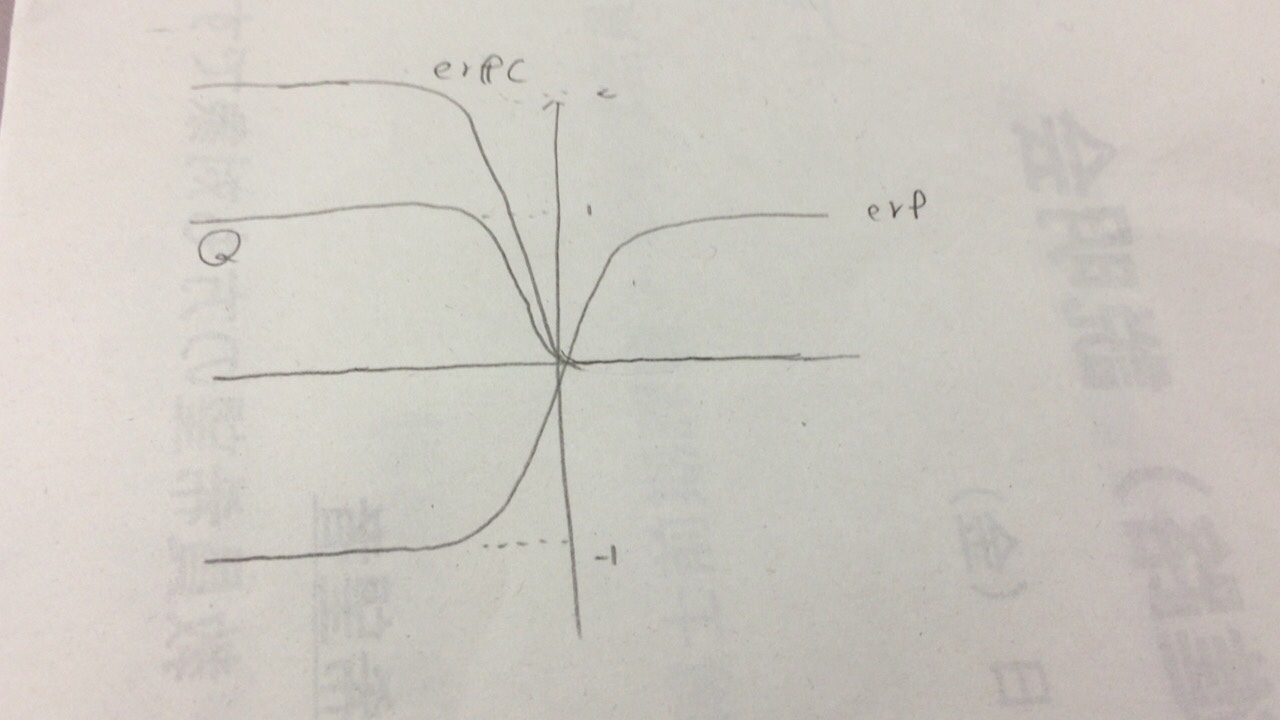
\includegraphics[width=5cm]{11_9_2.JPG}
		\end{center}
		●$erf(-x)=-erf(x)$→奇関数\\
		●$Φ(x)=\frac{1}{2}[1+erf(\frac{x}{\sqrt{2}}]=\frac{1}{2}erfc(-\frac{x}{\sqrt{2}})$\\
		●$erf(x)=2Φ(\sqrt{2}x)-1$\\
		●$erfc(x)=2[1-Φ(\sqrt{2}x)]$\\
		
\subsection{多次元確率変数}
	\subsubsection{同時確率分布}
		{\large{2変数の場合}}\\
		2つの離散型確率変数X,Yがあるとする。$X=x$であり、かつ、$Y=y$である確率
		\[
			P(X=x,Y=y)
		\]
		を2次元確率変数(X,Y)の{\textcolor{blue}{同時確率分布}}という\\
		※大文字X、Yは確率変数。小文字x,yは、その実現値である\\
		※$P(X=x,Y=y)=P_{XY}(x,y)=P(x,y)$と書くことがある\\
		
	\subsection{同時確率分布表}
		例・・・確率変数X,Yがどりらも0,1をとる場合
		\begin{center}
			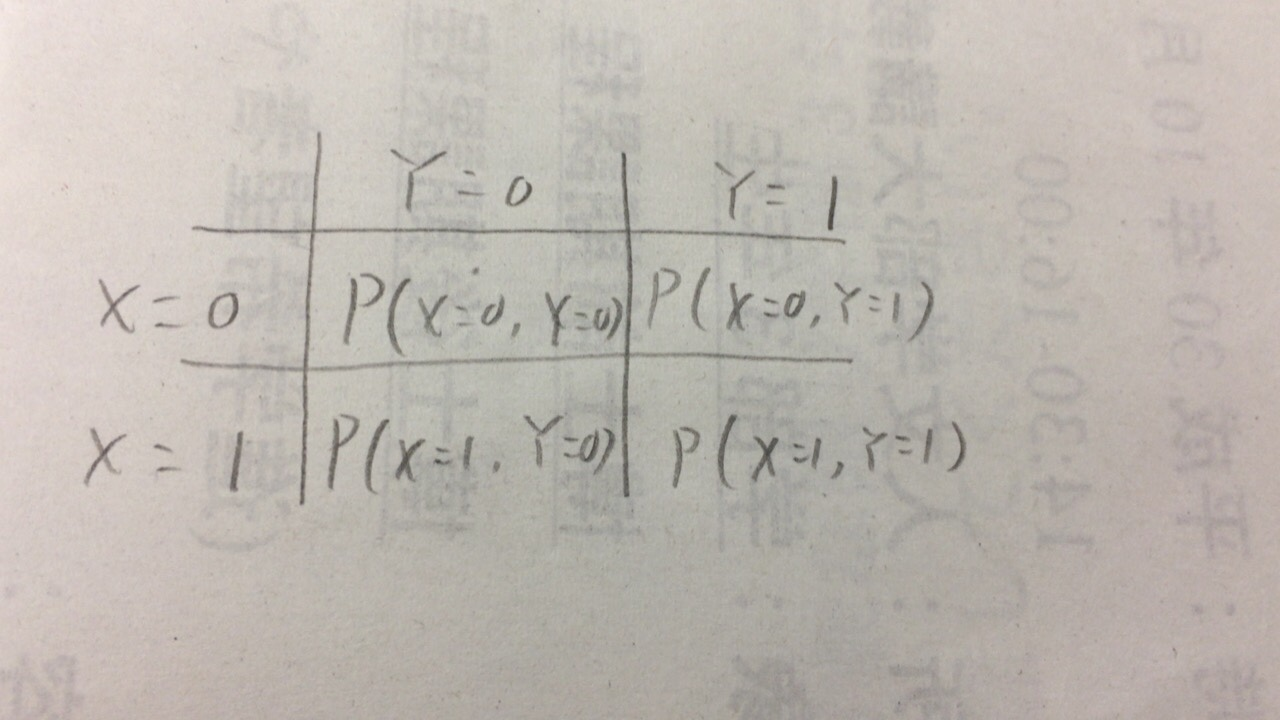
\includegraphics[width=5cm]{11_9_3.JPG}
		\end{center}
		ここで確率Pを全部足すと1となる
		
		{\large{n変数の場合}}
		n個の確率変数$X_1,X_2...X_n$があるとする\\
		各確率変数が
		\[
			X_i=x_i
		\]
		である\\
		確率分布
		\[
			P(X_1=x_1,X_2=x_2,...,X_n=x_n)
		\]
		をn次元確率変数の{\textcolor{blue}{同時確率分布}}という。\\
		※多変数の場合
		\[
			P(x_1,x_2...x_n)
		\]
		と書くことが多い
		ここで
		$x_i$が取り得るすべての場合について和を求めると1になる\\
		{\Large{例題}}\\
		2枚の大小の歪んだコインを同時に投げたとする。大きいコインの得点をX、小さいコインの得点をYで表すとする。\\
		大きいコインが表の時5点とし、裏のとき1点とする。\\
		小さいコインが表の時3点とし、裏の時0点とする。\\
		各コインの出方は次の同時確率分布の通りである。\\
		\begin{center}
			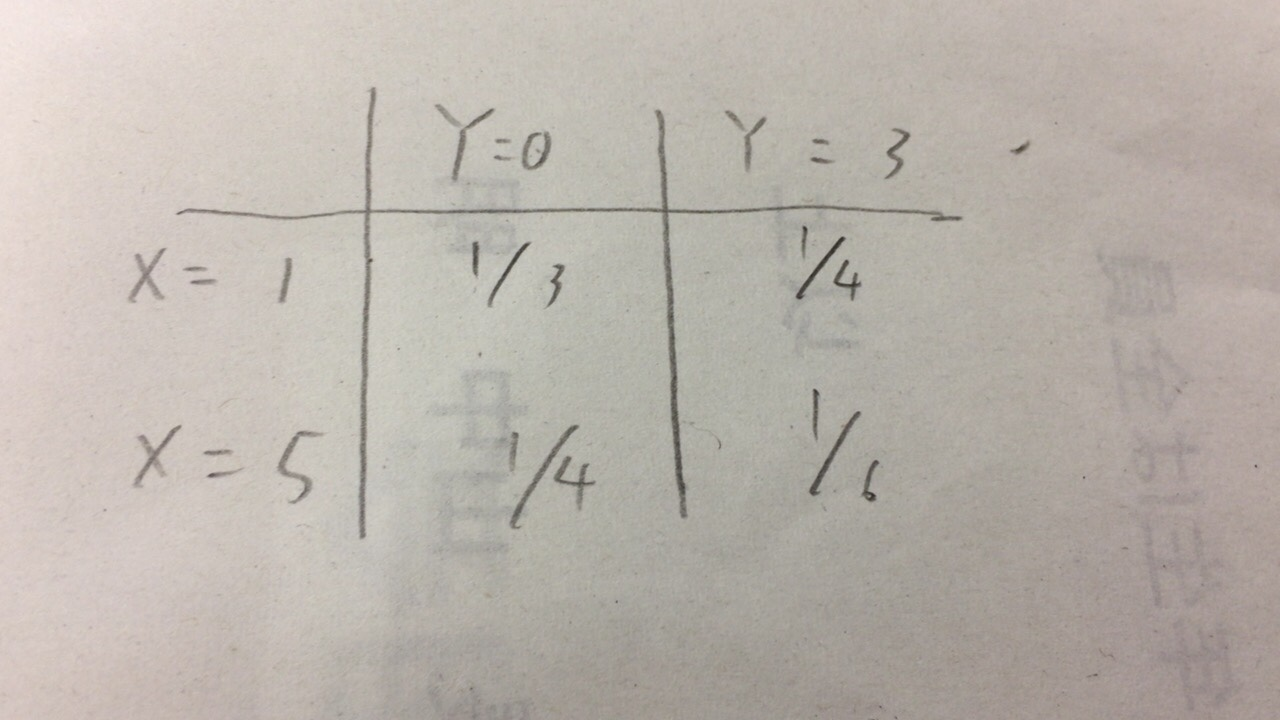
\includegraphics[width=5cm]{11_9_4.JPG}
		\end{center}
		この大小のコインの合計得点の期待値を求めなさい\\
		\begin{eqnarray}
			E[X+Y]=\sum_x\sum_y(x+y)P(X=x,Y=y)\\
			=(1+0)P(X=1,Y=0)+(1+3)P(X=1,Y=3)\\
			+(5+0)P(X=5,Y=0)+(5+3)P(X=5,Y=3)\\
			=\frac{47}{12}
		\end{eqnarray}
\section{11/30}
\subsection{同時確率分布}
	\begin{center}
		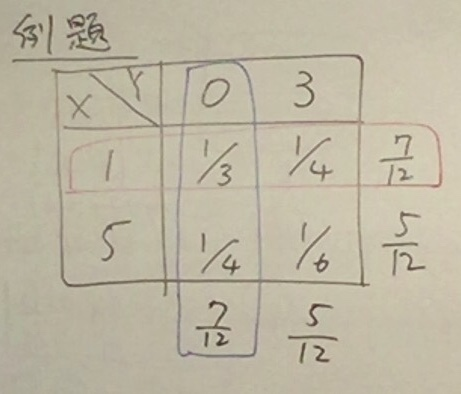
\includegraphics[width=5cm]{11_30_1.JPG}
	\end{center}
\subsection{周辺確率分布}
	同時確率分布が与えられた時、たとえば、$P(X=1)$はいくらか?\\
	X=1となるのは、Y=0でも、Y=3でもいいから、2つの確立の和になる\\
	\[
		P(X=1)=P(X=1,Y=0)+P(X=1,Y=3)=\frac{1}{3}+\frac{1}{4}=\frac{7}{12}
	\]
	***$(P=1)$を確率変数Xの周辺確率という.\\
	確率変数(X,Y)の同時確率分布において、確率変数Xの周辺確率分布は
	\[
		P(X=x)=\sum_y P(X=x,Y=y)
	\]
	で求められる。n変数の場合は
	\[
		P(X_1=x_1)=\sum_{x_2}\sum_{x_3}...\sum_{x_n}P(X_1=x_1,X_2=x_2,...,X_n=x_n)
	\]
	となる
\subsection{条件付き確率}
	例題において、\\
	Y=3であることがわかったとき、X=5である確率はいくらか\\
	この確率を
	\[
		P(X=5|Y=3)
	\]
	と表し、条件付き確率と呼ぶ\\
	Y=3は確定なので、同時確率分布表のY=3の列のみを見ればいい\\
	
	\[
		P(X=1)=P(X=1,Y=0)+P(X=1,Y=3)=\frac{1}{3}+\frac{1}{4}=\frac{7}{12}
	\]
	よって
	\begin{eqnarray}
		P(X=1|Y=3)=\frac{3}{5}\\
		P(X=5|Y=3)=\frac{2}{5}\\
	\end{eqnarray}
	確率変数(X,Y)において、ある事象Yが起こる条件のもとで、事象Xが起こる条件付き確率は
	\[
		P(X|Y)=\frac{P(X,Y)}{P(Y)}
	\]
	で求めることができる。\\
	以下の式から求めることができる。こっちの方が大事\\
	\begin{center}
		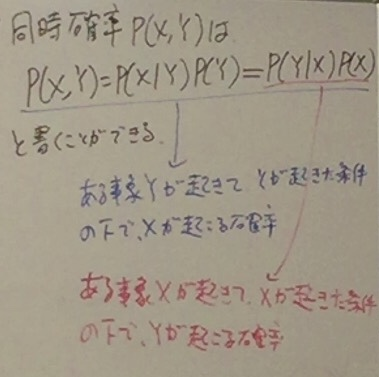
\includegraphics[width=10cm]{11_30_4.JPG}
	\end{center}
	これを覚えとけば上の式は導き出せる\\
	\subsubsection{例題}
	\begin{center}
		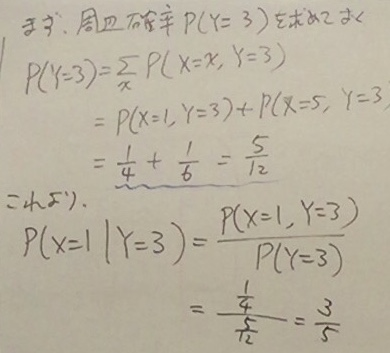
\includegraphics[width=7cm]{11_30_5.JPG}
	\end{center}
	これとおんなじようにしたら$P(X=5|Y=3)=\frac{2}{5}$がもとまる
\subsection{条件付き確率の期待値}
	\begin{center}
		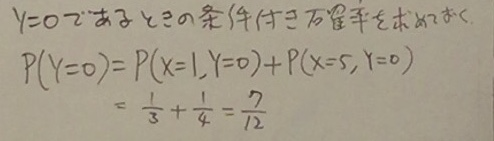
\includegraphics[width=7cm]{11_30_E.JPG}
	\end{center}
	\begin{center}
		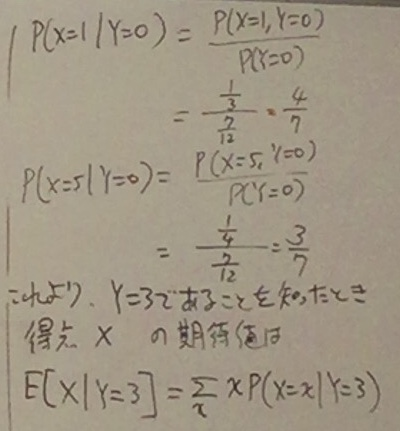
\includegraphics[width=7cm]{11_30_E2.JPG}
	\end{center}
	\begin{center}
		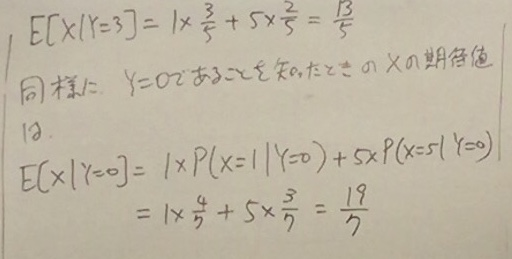
\includegraphics[width=7cm]{11_30_E3.JPG}
	\end{center}
	ここは絶対に試験に出る!!\\
	条件付き確率の意味をしっかり理解しておくこと
	
	\subsection{共分散}
	2つの確率変数X、Yの間に関連があれば、一方の結果は他方に影響する。\\
	{\Large{共分散}}\\
	\begin{center}
		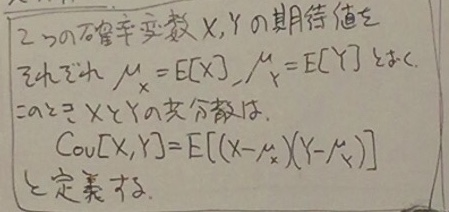
\includegraphics[width=7cm]{11_30_C.JPG}
	\end{center}
	Covはコバリアンスとよむ\\
	離散はくっついてないから足し算。連続だとくっついていわゆる面積になるから積分
	\begin{center}
		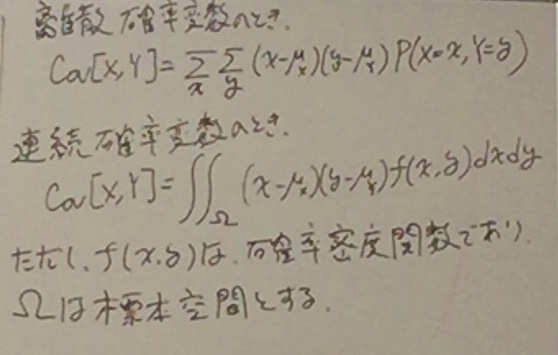
\includegraphics[width=7cm]{11_30_C2.JPG}
	\end{center}
	\begin{center}
		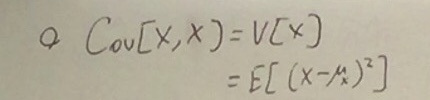
\includegraphics[width=7cm]{11_30_C3.JPG}
	\end{center}
	\subsection{計算公式}
	{\large{*********試験に式の証明の問題出るかも}}
	\begin{center}
		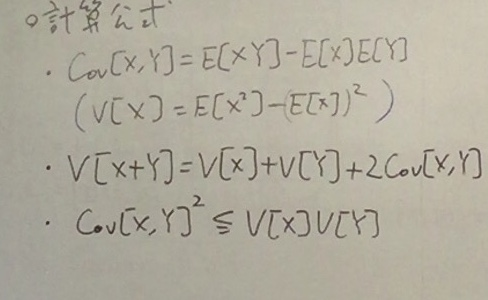
\includegraphics[width=7cm]{11_30_C4.JPG}
	\end{center}
	\subsection{分散共分散行列}
	多変数の場合の共分散は??\\
	確率変数$X_1,X_2,...,X_n$のi番目とj番目の共分散を
	\[
		σ_{ij}=Cov[X_i,X_j]
	\]
	とおく。これをまとめて行列で表したものを分散共分散行列という。これを大文字のシグマΣで表す\\
	\begin{center}
		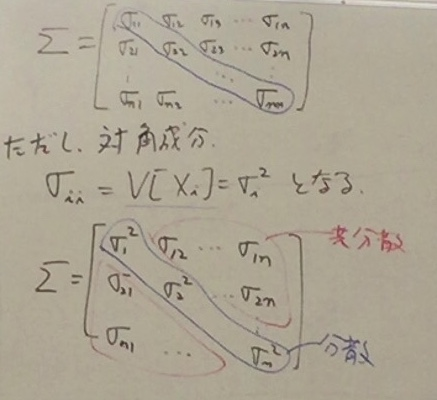
\includegraphics[width=7cm]{11_30_C5.JPG}
	\end{center}
	分散の式に等しい
	\subsection{相関係数}
	共分散を規格化した量\\
	\begin{center}
		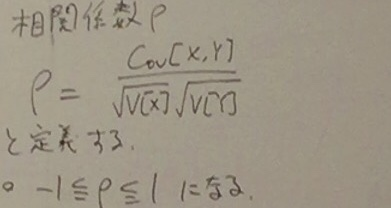
\includegraphics[width=7cm]{11_30_C6.JPG}
	\end{center}
	こう定義すると、$-1<ρ<1$となり、正規化される。\\
	$ρ=0$のとき、XとYは無相関(関係がない)である\\
\end{document}
	
	
	
	
	
	
	
	
	
	
	
	
	
	
	
	
	
	
	
	
	
	
	
	
	
	
	
	
	
	
	
	
	
	
		